\section{Introduction}

\subsection{Context-aware ASR}
General-purpose speech recognizers favour frequent words and rarely see names, product terms or technical
vocabulary during training. These rare words are exactly what a user cares about: a contact name,
a drug name, a term on a slide. Context-aware ASR feeds such information to the recognizer at run time
(a list of words or entities, the dialogue history, or text from slides) and expects the transcript
to contain the words of the context when they are spoken~\cite{pundak2018,zhao2019}.
Because the context changes with each user or call, retraining the model for every list is not an option.

\paragraph{Example.} The audio says ``call Siobhan'' and the contact list contains \emph{Siobhan}, \emph{Sean} and \emph{Anna}.
A plain system may write ``call shiv on'', because the name is rare and its spelling does not follow common patterns.
A context-aware system should write ``call Siobhan''. If the context is forced too strongly, the same system writes
``Siobhan'' even when the speaker said ``Sean''. This is a false alarm (over-biasing), and a good method must
reduce errors on listed words without causing it.

\paragraph{Metrics.} Besides the overall word error rate (WER), the field reports
B-WER and U-WER, the WER computed only on words that are, or are not, in the bias list~\cite{le2021triebias},
and R-WER, the share of listed-word tokens recognized wrongly. Phrase-level precision, recall and F1,
named-entity error rates (NE-WER, NE-CER) and the false-alarm rate are also common.
Definitions differ between papers, so numbers are compared only under the same setup.

\subsection{Taxonomy of approaches}
We organize the methods by \emph{where} the context enters the recognition pipeline (Fig.~\ref{fig:taxonomy}).
This grouping is our own synthesis and is not a standard of the field.
\begin{description}[leftmargin=1.2em,style=unboxed]
  \item[A. Decoding-time biasing.] The model is untouched. The list is compiled into a trie or FST
    and adds a bonus score during beam search (shallow fusion)~\cite{zhao2019,le2021triebias}.
  \item[B. In-model biasing.] The model takes the list as an extra input and is trained to use it:
    B1 adds a dedicated module (bias encoder, pointer-generator, copy mechanism)~\cite{pundak2018,lin2024copyne};
    B2 puts the context in the prompt of a speech LLM.
  \item[C. Post-recognition correction.] ASR runs as usual, then a second step compares the output with
    the list and fixes errors (word spotting, spelling correction, LLM-based correction)~\cite{andrusenko2024ctcws}.
  \item[D. Supporting techniques.] D1 retrieves a few likely candidates from a long list and passes them to A, B or C~\cite{gong2025brasr,mittal2025recast};
    D2 adapts the model itself (fine-tuning, LoRA, test-time adaptation).
\end{description}

\begin{figure}[h]
\centering
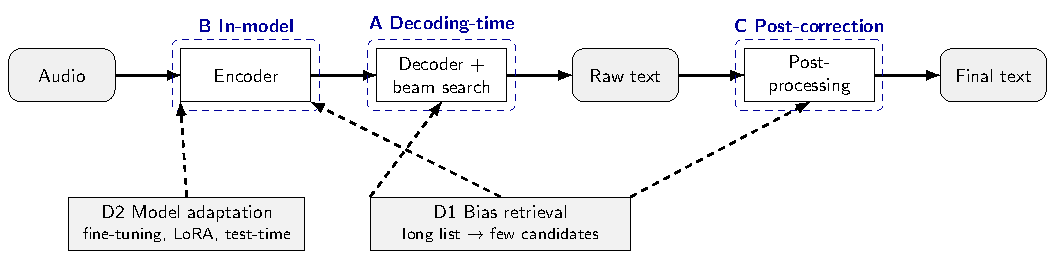
\includegraphics[width=\textwidth]{taxonomy.pdf}
\caption{Where context enters the ASR pipeline. Solid arrows: the recognition flow; dashed arrows: D1 and D2 support A--C.}
\label{fig:taxonomy}
\end{figure}

\subsection{Scope and contributions}
The project follows the research direction. We make four contributions.
\begin{enumerate}
  \item A survey of context-aware ASR across groups A--D, covering papers from A/A* conferences and Q1/Q2 journals
    of the last 3--5 years, each summarized with its strengths and weaknesses (Section~\ref{sec:survey}).
  \item A runnable demo of CopyNE~\cite{lin2024copyne}, with our own numbers set next to the author-reported ones (Section~\ref{sec:exp}).
  \item An ablation study on the same system (Section~\ref{sec:exp}).
  \item An in-depth analysis of one solution with a proposed improvement (Section~\ref{sec:analysis}).
\end{enumerate}
We found no Vietnamese study that targets contextual biasing in groups A--C directly, so the survey also notes
what is missing for Vietnamese. This search is preliminary and does not prove that none exists.
